\documentclass[12pt]{article}
\usepackage{amsfonts}
\usepackage{amsmath}
\usepackage{graphicx}
\usepackage{float}
\begin{document}
\title{Electrical Engineering 141, Homework 1}
\date{January 18th, 2019}
\author{Michael Wu\\UID: 404751542}
\maketitle

\section*{Problem 1}

\paragraph{a)}

Three feedback systems would be a thermostat, a Segway, and GPS software.

\paragraph{b)}

In this block diagram for a thermostat, the plant is the room that the thermostat is located in.
The input is a desired temperature, and the output is the actual temperature of the room. The sensing
mechanism is a thermometer that checks the actual temperature of the room. This is fed back to the control
mechanism which is a controller that turns the heating or cooling on. The heating and cooling components are
the actuating mechanism that acts to change the room's temperature. Possible disturbances that act on the
room come from the environment. For example, if it is a sunny day then the room will tend to be hotter. If it
is windy and a window is open, then the room may become colder.
\begin{figure}[H]
    \begin{center}
        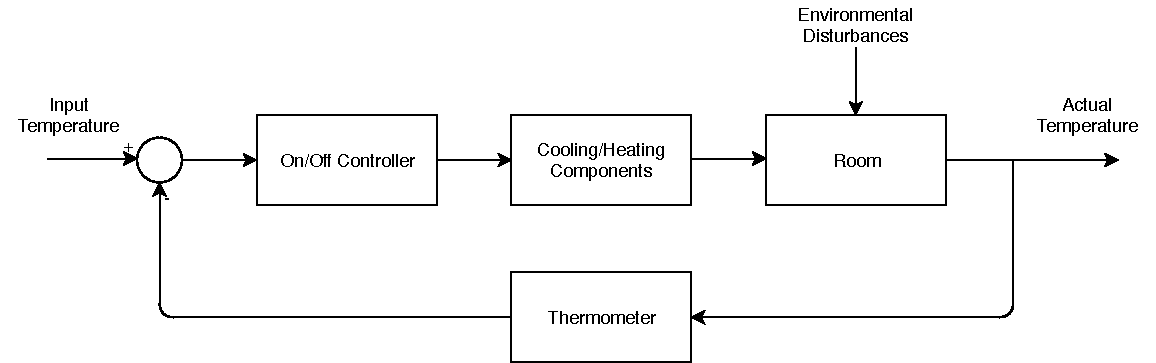
\includegraphics[width=5.3in]{Thermostat.pdf}
    \end{center}
\end{figure}

In this block diagram for a Segway, the plant is the Segway itself. The input is a balanced state, as the Segway
wants to not fall over. The output is the actual balance of the Segway. The sensing mechanism uses gyroscopes in
the Segway to detect the actual balance. This is fed to the control mechanism, the motor controller, which decides
whether to activate the motor forwards or backwards. The motor is the actuating mechanism, since it acts upon the
Segway to maintain balance. Possible disturbances include external forces from uneven ground or the rider's weight.
\begin{figure}[H]
    \begin{center}
        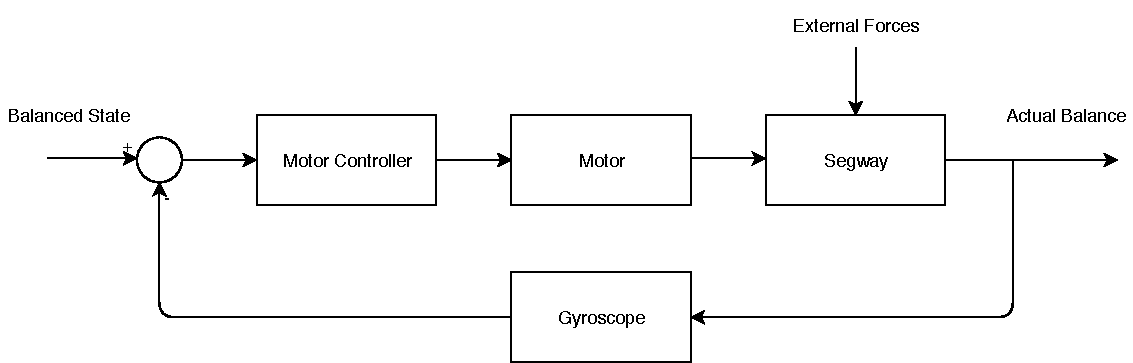
\includegraphics[width=5.3in]{Segway.pdf}
    \end{center}
\end{figure}

In this block diagram for a GPS system, the plant is the car that the GPS is guiding. The input is a target location,
and the output is the actual location of the car. The sensing mechanism is the position detector. This allows the GPS
unit to calculate directions, which is the control mechanism. The driver of the car listens to the directions in order
to move the car correctly, so the driver is the actuating mechanism. Possible disturbances include road hazards, traffic,
and other distractions that may force a detour or cause the driver to take a wrong turn.
\begin{figure}[H]
    \begin{center}
        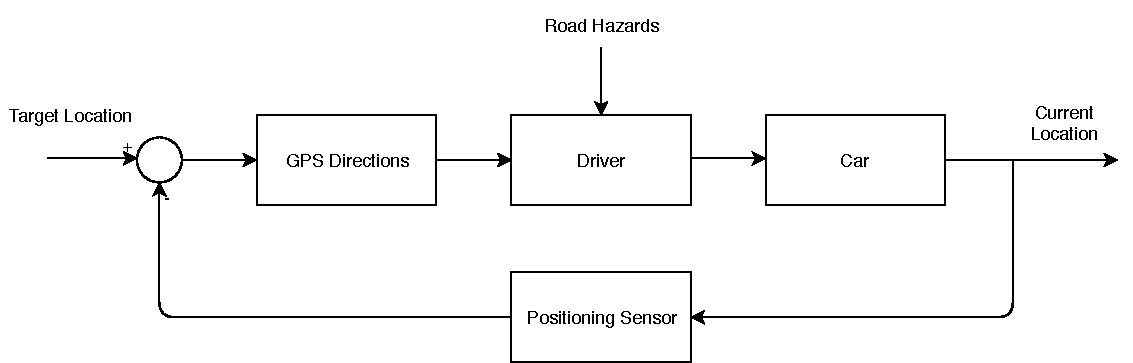
\includegraphics[width=5.3in]{GPS.pdf}
    \end{center}
\end{figure}

\paragraph{c)}

In these examples, the thermostat and segway use automatic control. The GPS system uses manual control since a human must
drive the car. All these systems are single-input-single-output. The thermostat and GPS are tracking systems, since they
attempt to match the output signal to the input signal. For example if a thermostat could be programmed to sinusoidally vary
the temperature so it is hot during the day and cold during the night and the GPS could be set to follow a target vehicle.
The Segway is a regulator system, since the input is a fixed state and the system attempts to move back to this state.

\section*{Problem 2}

In this block diagram, the inputs are the camera movement and possible noise that shifts around the camera lens. The camera
movement acts on the camera body which changes the direction of the camera lens. The output is the lens direction. The sensing
mechanism is the pitch and yaw sensor, which senses movements from the camera body. There must also be a sensor that detects
the current lens direction. The control mechanism is the motor controller, which takes the current lens position and the
movement of the camera body to decide how to activate the lens motors. The lens motors are the actuating mechanisms, since
they move the camera lens in order to smooth out its change in direction.
\begin{figure}[H]
    \begin{center}
        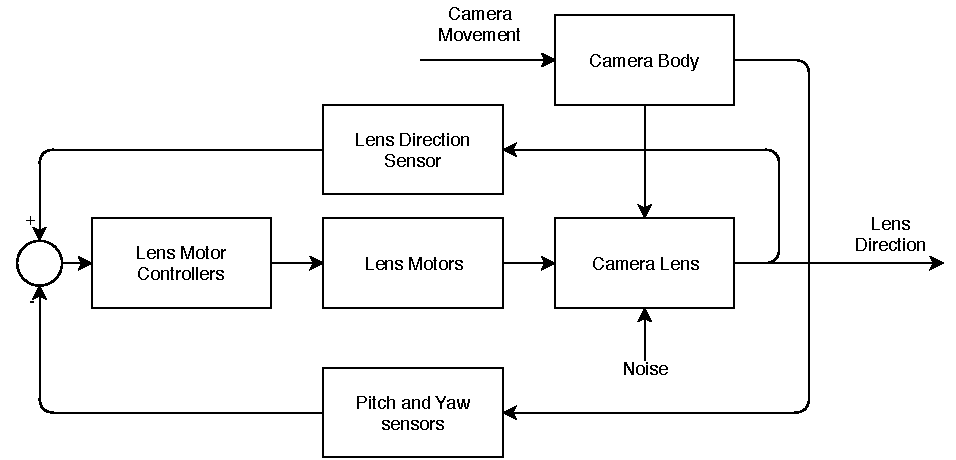
\includegraphics[width=5in]{Camera.pdf}
    \end{center}
\end{figure}

\section*{Problem 3}

\paragraph{a)}

The bilateral Laplace transform for \(x_1(t)\) is given by
\[\int_0^\infty e^{-(s+a)t}\, dt = \frac{1}{s+a}\]
and has a region of convergence for \(\mathbb{R}(s+a)>0)\). The bilateral Laplace transform for
\(x_2(t)\) is given by
\[\int_{-\infty}^0 -e^{-(s+a)}t\, dt = \frac{1}{s+a}\]
and has a region of convergence for \(\mathbb{R}(s+a)<0\).

\paragraph{b)}

We can rewrite this transfer function with Partial Fraction Expansion by using the factors \(s+3\) and
\(s-2\). This leads to the equivalent expression
\[H(s)=-\frac{1}{s+3} + \frac{1}{s-2}\]
Then the three regions of convergence are for \(\mathbb{R}(s)<-3\),  \(-3<\mathbb{R}(s)<2\), and
\(2<\mathbb{R}(s)\). These lead to the inverse transfer functions
\begin{align*}
    h_1(t)=\left(e^{-3t}-e^{2t}\right)u(-t) & \text{ for } \mathbb{R}(s)<-3\\
    h_2(t)=-e^{-3t}u(t)-e^{2t}u(-t) & \text{ for } -3<\mathbb{R}(s)<2\\
    h_3(t)=\left(-e^{-3t}+e^{2t}\right)u(t) & \text{ for } 2<\mathbb{R}(s)
\end{align*}
For an LTI system defined by the impulse response \(h_1(t)\), we obtain a system that is not causal since
the \(u(-t)\) term causes the impulse response to be nonzero when \(t<0\). It is also not stable since as
\(t\) goes to \(-\infty\), the response goes to \(\infty\) because of the \(e^{-3t}\) term. For an LTI
system defined by the impulse response \(h_2(t)\), we obtain a system that is not causal since
the \(u(-t)\) term causes the impulse response to be nonzero when \(t<0\). It is stable because for an input
bounded by \(\alpha\), we have that the output signal must be bounded by
\[\left|\alpha \left(\int_0^\infty-e^{-3t}\,dt + \int_{-\infty}^0 -e^{2t}\,dt\right)\right| = \alpha\frac{5}{6}\]
For an LTI system defined by the impulse response \(h_3(t)\), we obtain a system that is causal since the
\(u(t)\) term causes the impulse response to be zero when \(t<0\). It is also not stable since as
\(t\) goes to \(\infty\), the response goes to \(\infty\) because of the \(e^{2t}\) term.

\section*{Problem 4}

\paragraph{a)}

By applying the Final Value Theorem we have that if the limit
\[\lim_{t\to\infty} x(t)\] exists, then
\[\lim_{t\to\infty} x(t) = \lim_{s\to 0} sX(s)\]
so we obtain
\[\lim_{s\to 0} sX(s) = \lim_{s\to 0} \frac{s(2s^2+\omega^2)}{s(s^2+\omega^2)} = \frac{\omega^2}{\omega^2} =1\]
and therefore \(\lim_{t\to\infty} x(t) = 1\).

\paragraph{b)}

We can write the Laplace transform as
\[X(s) = \frac{s}{s^2+\omega^2} + \frac{1}{s}\]
which has the inverse Laplace transform of
\[x(t) = (\cos(\omega t)+1)u(t)\]
which oscillates around the limit 1 obtained in the previous section. In reality the limit
\(\lim_{t\to\infty} x(t)\) does not exist, due to the oscillation. So our previous conclusion is not
valid since the limit does not exist. To ensure that the Final Value Theorem holds, we must make sure that
our transfer function has only poles with negative real values so oscillations die out. The transfer
function can also include the pole \(s=0\), but cannot include purely imaginary poles.

\section*{Problem 5}

Because our system is a causal LTI system, the impulse response of this system must be zero for \(t<0\).
So if we have
\[\lim_{t\to 0^+} h(t) = 0\]
then the impulse response of this system will be continuous at zero. From the Initial Value Theorem, this
is equivalent to finding the limit
\[\lim_{s\to\infty} sH(s) = \lim_{s\to\infty}\frac{sb(s)}{a(s)} = 0\]
This limit is satisfied when the degree of \(a(s)\) is at least two higher than the degree of \(b(s)\),
which is a necessary and sufficient condition to conclude that the impulse response is continuous at 0.

\section*{Problem 6}

\paragraph{a)}

We know that the Laplace transform of our input is \(X(s)=\frac{1}{s-s_0}\). Then our output has the
Laplace transform
\[Y(s)=\frac{b(s)}{a(s)}\frac{1}{s-s_0} + \frac{I(s)}{a(s)}\]
Setting this equal to our desired form of
\[Y(s)=\frac{K_0}{s-s_0}+\frac{\beta(s)}{a(s)}+\frac{I(s)}{a(s)}\]
yields the equation
\begin{align*}
    \frac{K_0}{s-s_0}+\frac{\beta(s)}{a(s)}&=\frac{b(s)}{a(s)}\frac{1}{s-s_0}\\
    K_0+\frac{\beta(s)(s-s_0)}{a(s)}&=\frac{b(s)}{a(s)}\\
    K_0&=\frac{b(s)}{a(s)}-\frac{\beta(s)(s-s_0)}{a(s)}\\
    K_0&=\frac{b(s)-\beta(s)(s-s_0)}{a(s)}
\end{align*}
which gives us the value of \(K_0\). This also yields an expression for \(\beta(s)\) which is
\[\beta(s)=\frac{b(s)-K_0a(s)}{s-s_0}\]
Then because the numerator contains \(K_0\) times polynomial of degree \(n\), we can always choose
\(K_0\) so that the numerator is a polynomial with a degree greater than or equal to \(1\). After
dividing by \(s-s_0\) the remainder can have at most degree \(n-1\), so we can always write \(Y(s)\)
in our desired form. Then notice that the expression for \(K_0\) is not a function of \(s\). Then we
can evaluate it at \(s_0\) to obtain \(K_0=\frac{b(s_0)}{a(s_0)}=H(s_0)\). We can obtain the system response
\[y(t)=H(s_0)e^{s_0t}u(t)\]
if we have the transfer function
\[Y(s)=\frac{H(s_0)}{s-s_0}\]
which occurs when we set the initial values such that \(I(s)=-\beta(s)\). Since these two functions are
polynomials of the same degree \(n-1\), and we have \(n-1\) initial values that we can set, we have enough
degrees of freedom to always be able to set the initial values correctly.

\paragraph{b)}

If \(s_0\) is a zero of the transfer function, then \(K_0\) will be zero. So there will be no output component
of the form \(e^{s_0t}\), and the frequency \(s_0\) has effectively been blocked.

\paragraph{c)}

Since \(p\) is a pole of \(a(s)\), we know that \(a(s)\) can be evenly divided by \((s-p)\). In other words
\[a(s)=(s-p)\alpha(s)\]
where \(\alpha(s)\) is some polynomial of degree \(n-1\). Then we can choose initial conditions that satisfy the
condition \(I(s)=K\alpha(s)\) since \(I(s)\) is also a polynomial of degree \(n-1\). Then the Laplace transform
of our zero-input system response is
\[Y(s)=\frac{K}{s-p}\]
and we obtain the output
\[y(t)=Ke^{pt}u(t)\]
as desired.

\section*{Problem 7}

Taking the Laplace transform of both sides yields
\begin{align*}
    s^2Y(s)-sy(0^-)-y^\prime(0^-) + 6(sY(s) - y(0^-)) + 5Y(s) &= \frac{6}{s}\\
    s^2Y(s)-s-1+6sY(s)-6+5Y(s) &= \frac{6}{s}\\
    Y(s)(s^2+6s+5) &= \frac{6}{s}+s+7\\
    Y(s)(s^2+6s+5) &= \frac{s^2+7s+6}{s}\\
    Y(s) &= \frac{(s+1)(s+6)}{s(s+1)(s+5)}\\
    Y(s) &= \frac{s+6}{s(s+5)}\\
    Y(s) &= \frac{6}{5s} - \frac{1}{5(s+5)}\\
\end{align*}
Then taking the inverse Laplace transform yields
\[y(t) = \left(\frac{6}{5} - \frac{e^{-5t}}{5}\right) u(t)\]

\section*{Problem 8}

\paragraph{a)}

We know that the Laplace transform of the \(e^{-2t}\) term is \(\frac{1}{s+2}\). Then we must calculate the integral
\[\int_0^\infty t \cos(2t) e^{-st}\,dt\]
to and add these together to obtain the total Laplace transform. We can rewrite this integral as
\begin{align*}
    \int_0^\infty t \cos(2t) e^{-st}\,dt &= \int_0^\infty t \frac{e^{j2t}+e^{-j2t}}{2} e^{-st}\,dt\\
    &=\int_0^\infty t \frac{e^{(j2-s)t}+e^{-(j2+s)t}}{2}\,dt\\
    &=\left.\frac{t}{2}\left(\frac{e^{(j2-s)t}}{j2-s}-\frac{e^{-(j2+s)t}}{j2+s}\right)\right|_0^\infty\\
    &\qquad\qquad- \frac{1}{2}\int_0^\infty \frac{e^{(j2-s)t}}{j2-s}-\frac{e^{-(j2+s)t}}{j2+s}\,dt\\
    &=-\frac{1}{2}\int_0^\infty \frac{e^{(j2-s)t}}{j2-s}-\frac{e^{-(j2+s)t}}{j2+s}\,dt\\
    &=-\frac{1}{2}\left.\left(\frac{e^{(j2-s)t}}{(j2-s)^2}+\frac{e^{-(j2+s)t}}{(j2+s)^2}\right)\right|_0^\infty\\
    &=\frac{1}{2}\left(\frac{1}{(j2-s)^2}+\frac{1}{(j2+s)^2}\right)\\
    &=\frac{s^2-4}{(4+s^2)^2}
\end{align*}
So our final Laplace transform is
\[X(s)=\frac{1}{s+2} + \frac{s^2-4}{(4+s^2)^2}\]

\paragraph{b)}

\begin{align*}
    X(s) &= \int_0^\infty 4te^{-(4+s)t}\,dt\\
    &=\left.-4t\frac{e^{-(4+s)t}}{4+s}\right|_0^\infty + 4\int_0^\infty \frac{e^{-(4+s)t}}{4+s}\,dt\\
    &=4\int_0^\infty \frac{e^{-(4+s)t}}{4+s}\,dt\\
    &=\left.-\frac{4e^{-(4+s)t}}{(4+s)^2}\right|_0^\infty\\
    &=\frac{4}{(4+s)^2}
\end{align*}

\section*{Problem 9}

\paragraph{a)}

Using Partial Fraction Expansion we can rewrite the Laplace transform as
\[X(s)=-\frac{5}{2(s+1)} + \frac{5}{(s+1)^2} + \frac{5}{2(s+3)}\]
which has the inverse Laplace transform
\[x(t)=\left(-\frac{5}{2}e^{-t} + 5te^{-t} + \frac{5}{2}e^{-3t}\right)u(t)\]

\paragraph{b)}

Let's begin by finding the inverse Laplace transform of
\[\frac{s+2}{(s^2+0.4s+0.4)(s+1)(s+5)}\]
The expression \(s^2+0.4s+0.4\) has complex roots at \(-0.2\pm 0.6j\), so we can use Partial Fraction Expansion to rewrite this as
\[\frac{As+B}{s^2+0.4s+0.4}+\frac{C}{s+1}+\frac{D}{s+5}\]
where we have
\begin{align*}
    A&=-\frac{11}{39}\\
    B&=\frac{58}{195}\\
    C&=\frac{1}{4}\\
    D&=\frac{5}{156}
\end{align*}
The first term can be further rewritten as
\[A\frac{s+0.2}{(s+0.2)^2+0.6^2} + \frac{B-0.2A}{0.6}\frac{0.6}{(s+0.2)^2+0.6^2}\]
Then using our Laplace transform tables we can take the inverse which is
\[Ae^{-0.2t}\cos(0.6t)+\frac{B-0.2A}{0.6}e^{-0.2t}\sin(0.6t)+Ce^{-t}+De^{-5t}\]
Finally we can account for the \(100e^{-4s}\) term in \(X(s)\) by multiplying and shifting to yield
\begin{multline*}
    x(t)=\left(100Ae^{-0.2(t-4)}\cos(0.6(t-4))\right.\\
    +60(B-0.2A)e^{-0.2(t-4)}\sin(0.6(t-4))\\
    \left.+100Ce^{-(t-4)}+100De^{-5(t-4)}\right)u(t-4)
\end{multline*}
Plugging in for our constants yields
\begin{multline*}
    x(t)=\left(-\frac{1100}{39}e^{-0.2t+0.8}\cos(0.6t-2.4))\right.\\
    +\frac{276}{13}e^{-0.2t+0.8}\sin(0.6t-2.4)\\
    \left.+25e^{-t+4}+\frac{125}{39}e^{-5t+20}\right)u(t-4)
\end{multline*}

\section*{Problem 10}

\paragraph{a)}

\paragraph{b)}

\paragraph{c)}

\end{document}